\section{Date: 2026-11-10}
\noindent \textbf{Series ID: EF1T99XSLNQ} 

\noindent This series is titled Percent of Value of Loans Made Under Participation or Syndication by Size of Loan: (\$ Thousands) \$10 to \$99, Large Domestic Banks (DISCONTINUED) and has a frequency of Quarterly, 2nd Month's 1st Full Week. The units are Percent and the seasonal adjustment is Not Seasonally Adjusted.The observation start date is 2012-07-01 and the observation end date is 2017-04-01.The popularity of this series is 1. \\ 

\noindent \textbf{Series ID: IR41030} 

\noindent This series is titled Import Price Index (End Use): Household Appliances and has a frequency of Monthly. The units are Index 2000=100 and the seasonal adjustment is Not Seasonally Adjusted.The observation start date is 1984-12-01 and the observation end date is 2026-09-01.The popularity of this series is 3. \\ 

\subsection{Raw Regression}
\noindent Regresses the two series against each other directly. A significant result here can come just as easily from both series sharing a long-run trend as from any real relationship.

\begin{center}
\begin{tabular}{lclc}
\toprule
\textbf{Dep. Variable:}           & value\_fred\_IR41030 & \textbf{  R-squared:         } &     0.005   \\
\textbf{Model:}                   &         OLS          & \textbf{  Adj. R-squared:    } &    -0.050   \\
\textbf{Method:}                  &    Least Squares     & \textbf{  F-statistic:       } &   0.09834   \\
\textbf{Date:}                    &   Tue, 10 Nov 2026   & \textbf{  Prob (F-statistic):} &    0.757    \\
\textbf{Time:}                    &       18:58:16       & \textbf{  Log-Likelihood:    } &   -48.115   \\
\textbf{No. Observations:}        &            20        & \textbf{  AIC:               } &     100.2   \\
\textbf{Df Residuals:}            &            18        & \textbf{  BIC:               } &     102.2   \\
\textbf{Df Model:}                &             1        & \textbf{                     } &             \\
\textbf{Covariance Type:}         &      nonrobust       & \textbf{                     } &             \\
\bottomrule
\end{tabular}
\begin{tabular}{lcccccc}
                                  & \textbf{coef} & \textbf{std err} & \textbf{t} & \textbf{P$> |$t$|$} & \textbf{[0.025} & \textbf{0.975]}  \\
\midrule
\textbf{const}                    &     110.6895  &        1.199     &    92.314  &         0.000        &      108.170    &      113.209     \\
\textbf{value\_fred\_EF1T99XSLNQ} &      -0.0286  &        0.091     &    -0.314  &         0.757        &       -0.221    &        0.163     \\
\bottomrule
\end{tabular}
\begin{tabular}{lclc}
\textbf{Omnibus:}       &  1.232 & \textbf{  Durbin-Watson:     } &    0.197  \\
\textbf{Prob(Omnibus):} &  0.540 & \textbf{  Jarque-Bera (JB):  } &    1.035  \\
\textbf{Skew:}          & -0.357 & \textbf{  Prob(JB):          } &    0.596  \\
\textbf{Kurtosis:}      &  2.145 & \textbf{  Cond. No.          } &     25.0  \\
\bottomrule
\end{tabular}
%\caption{OLS Regression Results}
\end{center}

Notes: \newline
 [1] Standard Errors assume that the covariance matrix of the errors is correctly specified.

\begin{figure}
\centering
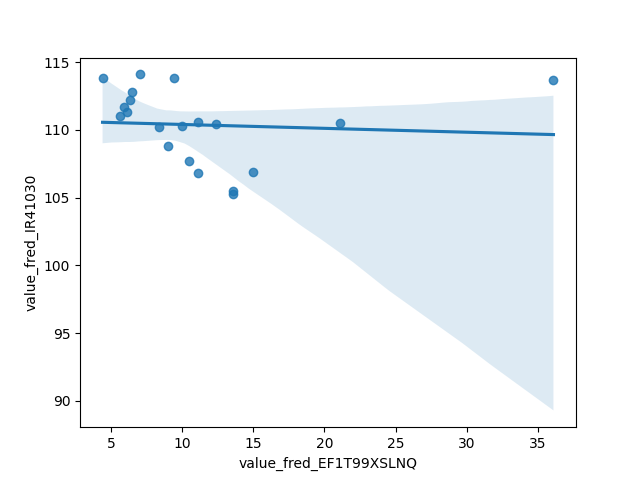
\includegraphics[scale = 0.9]{plots/plot_2026-11-10.png}
\caption{Raw Regression Plot for 2026-11-10}
\end{figure}
\newpage
\subsection{Detrended Regression}
\noindent Regresses the residuals of each series after removing its own linear time trend, so a shared trend can no longer drive the result on its own. A relationship that stays significant here is better evidence of a genuine link between the two series.

\begin{center}
\begin{tabular}{lclc}
\toprule
\textbf{Dep. Variable:}                      & value\_fred\_IR41030\_detrended & \textbf{  R-squared:         } &     0.011   \\
\textbf{Model:}                              &               OLS               & \textbf{  Adj. R-squared:    } &    -0.044   \\
\textbf{Method:}                             &          Least Squares          & \textbf{  F-statistic:       } &    0.1915   \\
\textbf{Date:}                               &         Tue, 10 Nov 2026        & \textbf{  Prob (F-statistic):} &    0.667    \\
\textbf{Time:}                               &             18:58:16            & \textbf{  Log-Likelihood:    } &   -31.490   \\
\textbf{No. Observations:}                   &                  20             & \textbf{  AIC:               } &     66.98   \\
\textbf{Df Residuals:}                       &                  18             & \textbf{  BIC:               } &     68.97   \\
\textbf{Df Model:}                           &                   1             & \textbf{                     } &             \\
\textbf{Covariance Type:}                    &            nonrobust            & \textbf{                     } &             \\
\bottomrule
\end{tabular}
\begin{tabular}{lcccccc}
                                             & \textbf{coef} & \textbf{std err} & \textbf{t} & \textbf{P$> |$t$|$} & \textbf{[0.025} & \textbf{0.975]}  \\
\midrule
\textbf{const}                               &    1.939e-12  &        0.275     &  7.04e-12  &         1.000        &       -0.579    &        0.579     \\
\textbf{value\_fred\_EF1T99XSLNQ\_detrended} &       0.0176  &        0.040     &     0.438  &         0.667        &       -0.067    &        0.102     \\
\bottomrule
\end{tabular}
\begin{tabular}{lclc}
\textbf{Omnibus:}       &  0.487 & \textbf{  Durbin-Watson:     } &    0.960  \\
\textbf{Prob(Omnibus):} &  0.784 & \textbf{  Jarque-Bera (JB):  } &    0.071  \\
\textbf{Skew:}          &  0.145 & \textbf{  Prob(JB):          } &    0.965  \\
\textbf{Kurtosis:}      &  3.008 & \textbf{  Cond. No.          } &     6.86  \\
\bottomrule
\end{tabular}
%\caption{OLS Regression Results}
\end{center}

Notes: \newline
 [1] Standard Errors assume that the covariance matrix of the errors is correctly specified.

\begin{figure}
\centering
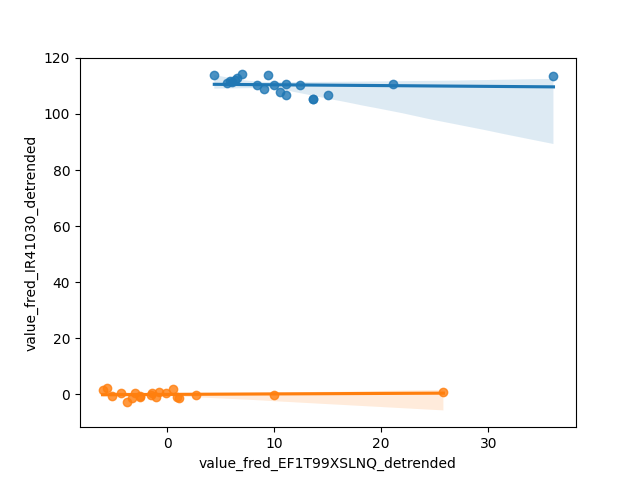
\includegraphics[scale = 0.9]{plots/plot_2026-11-10_detrended.png}
\caption{Detrended Regression Plot for 2026-11-10}
\end{figure}
\newpage
